\chapter{Generalized Compressive Sensing}
\index{Generalized Compressive Sensing@\emph{Generalized Compressive Sensing}}
\label{chp:generalized-cs}

In this chapter, we find the matrix tansformations to synchronize network data and show the benefit in missing value interpolation and activity recognition.

\section{Analysis of Network Matrices}

There are different factors that contribute to the lack of low rank structure in real data: (i) presence of measurement errors, noise, and anomalies, (ii) lack of synchronization across measurements (\eg, the original matrix may not be low-rank because the start time of the measurements across different elements are different, but after aligning them up, the new matrix may become low-rank), and (iii) lack of uniform speed (\eg, the raw samples of the same gesture performed at different time may not be low-rank due to different speeds of performing the gesture, but become similar after adjusting their speeds to the common one), and the combinations of these factors.

To validate our intuition, we study a range of network matrices. 
For each network matrix, we mean center each row (\ie, subtract from
each row its mean value) and apply singular value decomposition
(SVD) to examine if the mean-centered matrix has a good low-rank
approximation.  The metric we use is the fraction of total variance
captured by the top $K$ singular values, \ie, $\left({\sum_{i=1}^{K}
  s_i^2}\right)/\left({\sum_{i} s_i^2}\right)$, where $s_i$ is the
$i$-th largest singular value and $\left({\sum_{i} s_i^2}\right)$
gives the total variance of the mean-centered coordinate matrix.  Note
that $1 - \left({\sum_{i=1}^{K} s_i^2}\right)/\left({\sum_{i}
  s_i^2}\right)$ is the relative approximation error of the best
rank-$K$ approximation with respect to the squared Frobenius norm.

Figure~\ref{fig:sync-matrix-rank} plots the fraction of total
variance captured by the top $K$ singular values for different
traces. The smaller the value, the lower rank the matrix is.
As it shows, when the data is synchronized, the rank is 
7\% to 62\% lower than that when the data is unsynchronized.

\begin{figure}[h!]
  \centering
  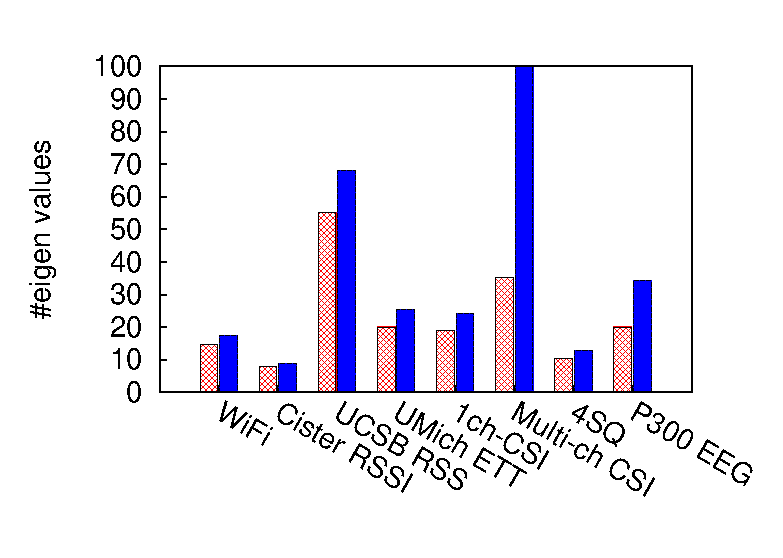
\includegraphics[width=1\figurewidthA]{fig_gen/rank.shift.eps}
  % \caption{CDF of energy that are contained in the top K singular values
  %   of synchronized and unsynchronized traffic matrices.}
  \caption{CDF of ranks of synchronized and unsynchronized data.}
  \label{fig:sync-matrix-rank}
\end{figure}


\section{Our Approach}

Based on the analysis results, we classify the data into the following types and propose to develop a generalized compressive sensing to support all of them:
\begin{enumerate}
\item The original matrix are close to low-rank.

\item The matrix after removing anomalies/noise is close to low-rank.

\item The matrix after temporal shift becomes close to low-rank.

\item The matrix after uniform stretch/compression becomes close to low-rank.

\item The matrix after temporal shift and uniform stretch/compression becomes close to low-rank.
\end{enumerate}

The existing work focuses on (1). To support (2), we develop LENS decomposition as shown in Chapter~\ref{chp:robust-cs}. To support (3), we use cross correlation to identify the shift that maximizes correlation coefficient and then align the data according to the shift before further analysis. Note that the shift can be identified even when there are missing elements since cross correlation can be computed based on the known entries. To extend beyond two rows, we can first perform pairwise cross correlation and derive affinity matrix $A(i, j)$, where $(i, j)$-th entry denotes the cross correlation between the $i$-th and $j$-th elements. Then we use spectral clustering to cluster the data, where each cluster contains multiple rows. We then pick the best row such that the remaining rows after shifting can maximize the total cross correlation. The best row from each cluster represents a major feature and can be used for pattern matching. The insight that shifting may help reduce the rank of the matrix enables us to apply compressive sensing to matrices that are not close to low-rank in the original form.

To support (4), we can search for a scaling factor that maximizes the cross correlation between a pair of data. As in (3), we first cluster the data based on the affinity matrix derived after performing pairwise stretch/compression, and then find the representative for each cluster. To support (5), we search for a combination of scaling factor and stretch for each pair of data and derive an affinity matrix accordingly. Then again we can cluster based on the affinity matrix and find a representive for each cluster. 

\section{Applications}

\para{Missing Value Interpolation}: 
We can apply generalized compressive sensing to support missing value interpolation, prediction, anomaly detection, compression, and pattern matching. Our approach is likely to out-perform existing compressive sensing approaches because the original matrices are relatively high rank and directly applying compressive sensing do not work well.

\para{Activity Recognition}: 
We can support the application for activity recognition. The reason that DTW is difficult to support the other network applications is that performing general warping requires knowing the complete data, whereas the shift and stretch can be found even when some elements are missing. The benefits of our approach over existing classification method is that, after synchronization, multiple subjects perform the same activity at the same time so we can utilize the group information to improve the recognition accuracy. One intuitive way to utilize the group information is to do majority vote among subjects. 

\section{Conclusion and On-going Work}
In this chapter, we observe that real-world data may not be low rank due to lack of synchronization and uniform speed. We propose a method to find the matrix transformations to synchronize and stretch/compress network data. There are many applications for the matrix transformations. In our futurer work, we plan to do extensive evaluation to show the benefit in missing value interpolation and activity recognition.

